\documentclass[main]{subfiles}

\begin{document}

    The IPS is composed of 3 main blocks:
    \begin{itemize}
        \item A Transmitting coil ({\bf TX Coil})
        \item Two or more Receiving coils ({\bf RX Coils})
        \item A rotating Target
    \end{itemize}

    \begin{figure}[h]
        \centering
        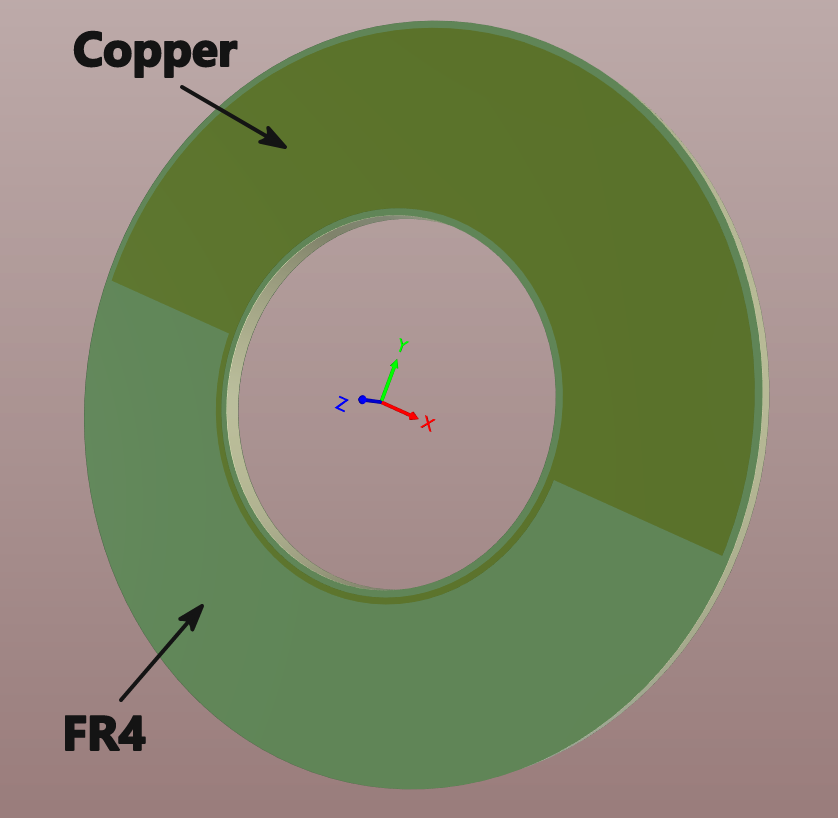
\includegraphics[width=0.5\linewidth]{img/target_1pp.png}
        \caption{Target example}
        \label{FIG_TARGET_1PP}
    \end{figure}

    \begin{figure}[h]
        \centering
        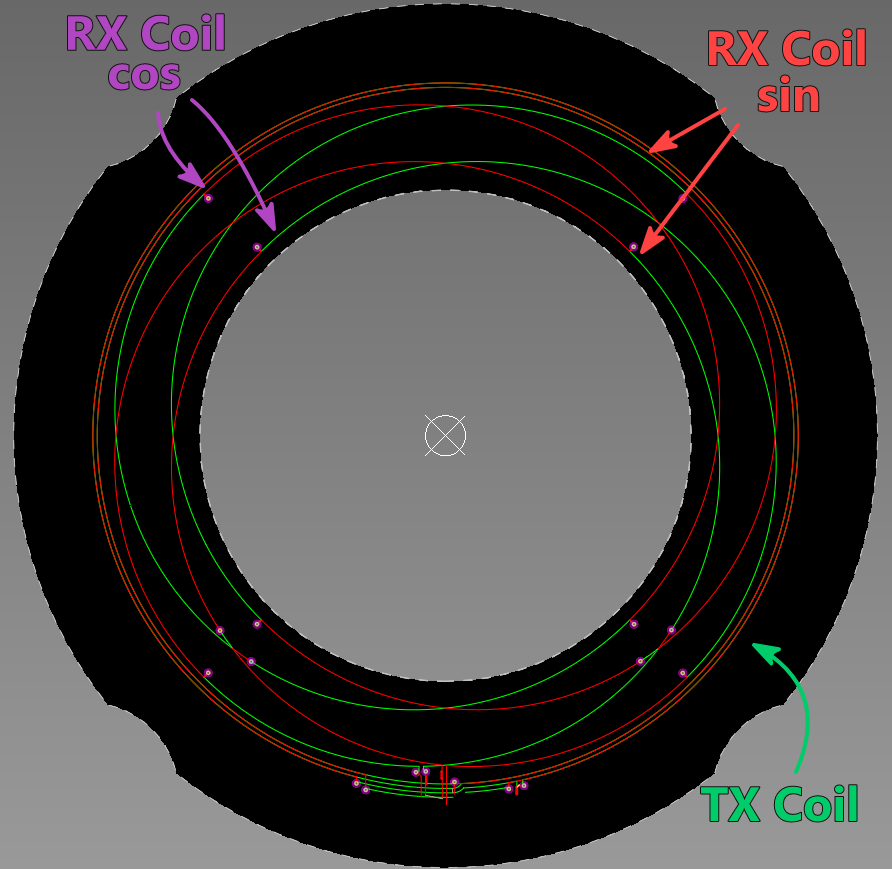
\includegraphics[width=0.5\linewidth]{img/pcb_coil_1pp.png}
        \caption{Pcb coil board example}
        \label{FIG_COIL_PCB_1PP}
    \end{figure}

    Usually the TX and RX coils are created on a single PCB (figure \ref{FIG_COIL_PCB_1PP}), 
    which is mounted on the stationary side of the sensor; while the target can 
    be realized on another PCB or using another piece of conducting material.

    To work properly the target should rotate above the PCB coils, around those 
    coils axis.

    The target can be obtained dividing a circular area into evenly sized angular 
    sectors, which will be filled with conductive material or air alternately
    (Figure \ref{FIG_TARGET_1PP}).

    To detect the position, a high frequency ($1MHz$ to $5 MHz$), sinusoidal 
    magnetic field is produced, by the current which flows through the TX coil.
    When the magnetic field reaches the conductive material of the target it induces 
    Eddy currents in it. Those currents oppose to the magnetic field, practically acting 
    as a shield.

    RX coils have a variable radius as a function of the angle, in order to 
    modulate the magnetic flux linkage (and the induced voltage) with the position 
    of the target.
    For example they can have a radius which makes sinusoidal oscillations around 
    its mean value, to produce sinusoidal waveforms when the target spins at a 
    constant speed.

    The key point is that the RX coils are designed in a differential way:
    at the angle at which the positive path of the coil hits its maximum radius, the return 
    path has its minimum radius; since the return path is connected in series with
    the positive one, and it links the flux in the opposite direction, the net 
    flux linkage of the coil is doubled and the same happens to induced voltage.

    Usually there are two sinusoidal coils which are $90^\circ$ spaced, to 
    produce sine and cosine signals.

    The received signals are AM modulated  they need a demodulation to obtain 
    pure sinusoidal signals.

    This task is often carried out along with exitation by a dedicated IC, so
    that synchronous demodulation can be performed.
    
\end{document}